\documentclass{article}
\usepackage[utf8]{inputenc}
\usepackage{graphicx}
\graphicspath{{./imgs/}}

\title{Multiple Round Ballot Polling Risk-Limiting Audit Simulations}
\author{ }
\date{ }

\begin{document}

\maketitle

\begin{abstract}
    Risk-Limiting Audits (RLAs) guarantee with known probability 
    that if the outcome of an 
    election is incorrectly announced, it will be detected, 
    and a full hand recount will be performed. 
    In Ballot-polling RLAs, samples of ballots are drawn and tallied.
    In this paper we present an audit simulation framework
    that can be used to confirm theoretical results of audits.
    We present such experimental results for multiple round 
    ballot-polling RLAs.
    BRAVO [citation] has long been the standard ballot-polling RLA,
    while Minerva was recently introduced with the claim
    that fewer ballots on average are necessary to conclude 
    an audit.
    [Minerva paper] presented experimental
    results for one round audits, and here
    we present results
    from simulations of multiple round audits using Minerva 
    as well as BRAVO 
    (both Selection-Ordered 
    BRAVO and End-of-Round BRAVO).
    The simulation results agree within reasonable error with
    the mathematical properties claimed in [Minerva paper].
    On average, BRAVO audits are unnecessarily conservative 
    while Minerva audits stop with fewer ballots. We also
    present details on software implementing Minerva and
    the simulations themselves.
\end{abstract}

\section{Introduction: B2 and R2 Ballot Polling RLAs}
In ballot-polling RLAs, samples of ballots are drawn and tallied
in rounds
after each of which a statistical measure determines whether to
continue. 
Some ballot-polling audits (B2 audits) 
are designed to make a stopping decision
after each individual ballot is sampled.
Other ballot-polling audits (R2 audits) assume many ballots are drawn
at once and make a stopping decision at the conclusion of each 
so-called round.
In practice, election officials draw many ballots at once.
For this reason, R2 audits are used or B2 audits are applied to 
rounds.
BRAVO is a B2 audit. 
When an audit is performed in rounds, BRAVO can have its
stopping condition applied once at the end of each round
(End-of Round (EoR) BRAVO).
This method ignores the possibility of stopping earlier in the 
sample and thus requires more ballots on average to sample.
Alternatively, the order of ballots in the sample can be tracked
by election officials and the B2 BRAVO stopping condition can 
be applied retroactively to all subsamples 
(Selection-Ordered (SO) BRAVO).
SO BRAVO requires fewer ballots on average than EoR BRAVO but
requies the work of tracking the order of ballots rather than
just their tally.
Minerva was designed for R2 audits and applies its stopping rule
once for each round.
Minerva, by design then, requires fewer ballots to be sampled when 
an audit is performed in rounds.
 
\section{Simulations to Confirm Theoretical Results}

The outcomes of RLAs depend on random chance; some random samples
support the alternative hypothesis more than expected, resulting in 
quick low-risk conclusions, while other unlucky samples require subsequent
rounds to confirm the announced results.
We can simulate random samples for various underlying ballot 
distributions by computing pseudorandom samples. 
By applying an audit's stopping condition to thousands of such
simulated samples, the average behavior of the simulated
audits will tend towards the true behavior of the audit.
In this way, we can examine whether theoretical claims about an audit are
actually correct.

For this paper, we simulated audits for 
the 2020 Presidential election
in all US states whose margin was at least $5\%$.
Round sizes increase roughly proportional to the inverse
square of the margin, so 
smaller margins are computationally more expensive to simulate.
For each of these states, we simulated 
$10,000=10^4$ audits with the announced
underyling ballot distribution
and an additional $10,000=10^4$ audits with a tie
as the underlying ballot distribution.
These are reasonable choices for inital simulation experiments
because most audits frame the stopping decision as a binary
hypothesis test where the null hypothesis assumes an underyling tie
and the alternative hypothesis assumes the announced distribution.
A standard first round size in ballot-polling audits
has been one which achieves a $90\%$ probability
of stopping, and we chose round sizes to reflect this standard
in our simulations.
We ran our simulations for up to five rounds.
With a $90\%$ stopping probability, 
an audit only has a $a$ probablity of not stopping
by the end of the fifth round, assuming the outcome was correctly
announced.


\subsection{End-of-Round BRAVO}
For the EoR BRAVO simulations, our software estimated for each round
the round size that would achieve a $90\%$ probability of stopping.
For the simulations with the announced outcome as the underlying
ballot distribution, for each round $j$ we computed the probability
of stopping given that an audit had continued through round $j$.
That is, among the audits remaining at the beginning of round $j$, 
we found the proportion which then stopped in round $j$.
%This metric shows whether our software accurately estimated the minimum number of ballots that achieve the $90\%$ probability of stopping.

%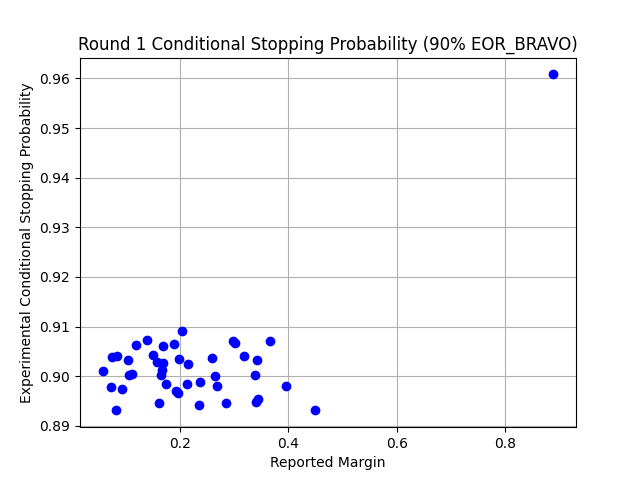
\includegraphics[scale=.6]{eor_bravo_90perc_10^4_corrected/cond_sprob/r1_cond_sprob.png}
\begin{center}
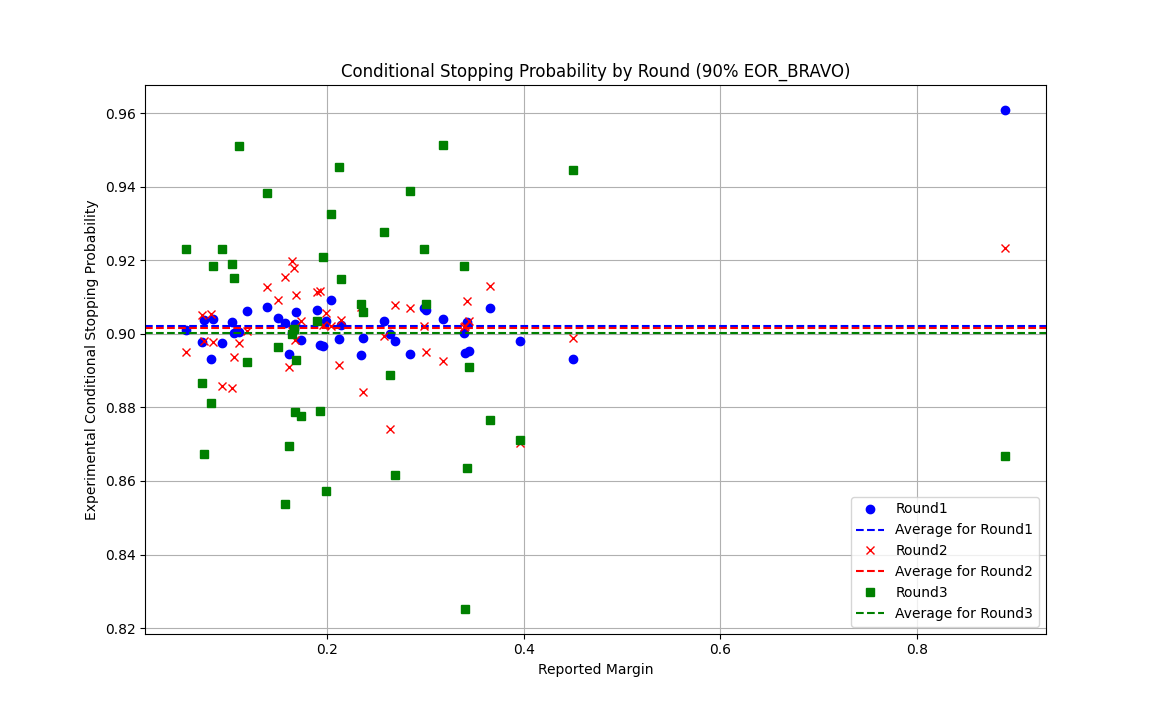
\includegraphics[scale=.41]{eor_bravo_90perc_10^4_corrected/cond_sprob_first_3_rounds.png}
\end{center}
[Figure 1] shows the proportion of audits that stopped in the $j$th round
to all audits which had not already stopped in a preceding round.
This proportion is shown for each state whose margin is given on the 
horizontal axis.
Here we display only the first three rounds
since very few audits, $(.1)^{j-1}$ on average, 
make it to the $jth$ round, 
and as a result the data becomes exponentially less representative
of the true probabilities.

The proportion shown in [Fig 1] gives an estimate
of the true probability of an EOR BRAVO audit stopping in the $j$th round,
given that it has not already stopped in a previous round. 
In [Figure 1] we see that, especially in earlier rounds for which 
the values are more representative of true audit behavior, 
our predictions are accurate.
In particular the average across all margins is just above $.9=90\%$ for
all three rounds.

The total risk across all $5$ rounds for this audit is arguably
the most important metric to consider.
The risk of an audit is the probability that the audit
stops despite an underlying tie. 
%That is, the risk $R$ of audit $\mathcal{A}$ is 
%$$R(\mathcal{A})=Pr[\mathcal{A}=\text{Correct}\mid H_0].$$
Therefore, we now consider the proportion of audits with an underlying
tie.

%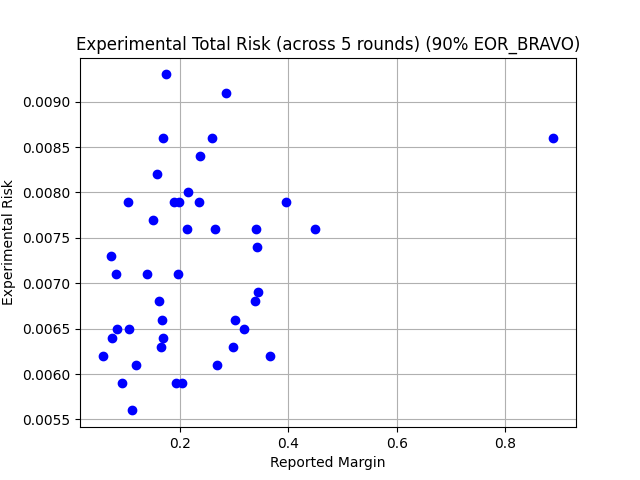
\includegraphics[scale=.5]{eor_bravo_90perc_10^4_corrected/total_risk.png}
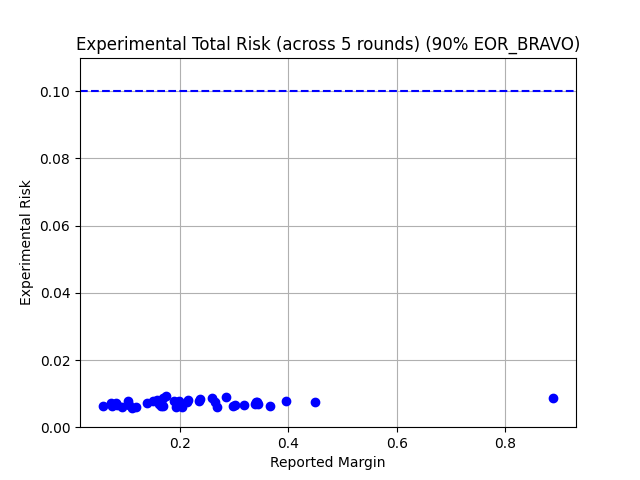
\includegraphics[scale=.7]{eor_bravo_90perc_10^4_corrected/total_risk_with_alpha.png}

[Fig 2] shows, for each state margin,
the proportion of EOR BRAVO audits with an underlying
tie which stopped before the conclusion of the $5$ rounds to the 
total number of audits, $10^4$.

[Fig 2] makes it clear that the risk of EOR BRAVO is roughly
an order of magnitude less than the risk limit. 
That is, on average, roughly $10$ times more audits could have stopped 
with the audit still meeting the risk limit.
These simulations support the claim made in [Minerva paper]
that EOR BRAVO is unnecessarily conservative and thus requires
more ballots on average.


% \subsection{Selection-Ordered BRAVO}
% next_sample_size code is slow... tie simulations running still

\subsection{Minerva}
For Minerva, it has not been shown that round sizes can be chosen
during the audit. That is, an adversary with knowledge of the history
of the audit may be able to choose round sizes which cause the 
risk of the audit to exceed the risk limit.
For this reason, we have to choose the round sizes of a Minerva 
audit a priori.
For this paper, we consider two choices of round sizes.
For both, we estimate and then use the minimum first round size 
which achieves
a $90\%$ probability of stopping.
Then, for subsequent rounds, we either (i) 
draw the same number of ballots in each round or (ii)
multiply the previous round size by a factor of $1.5$ and 
sample this many new ballots.
We consider the case of drawing samples of the same size
because it may reflect a practical way to continue an
audit; if election officials have selected some first round size within
reasonable logistical bounds, drawing the same number of 
ballots in subsequent rounds may be practical.
We also consider round sizes with samples increasing by a multiple
of $1.5$ because this multiple gives a very rough approximation of 
round sizes with a $90\%$ probability of stopping.

\subsubsection{Round Sizes with Multiple of $1.0$}

As with the preceding simulations, we ran $10,000=10^4$ trials
per state for both the underlying tie and underlying announced
outcome.

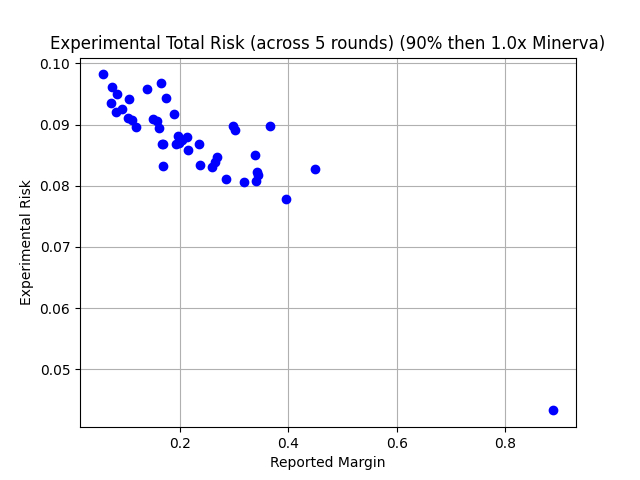
\includegraphics[scale=.7]{minerva_multiround_1x_10^4/total_risk.png}

[Fig above] shows that all simulations had a risk of less than 
$.1$, the risk limit. 
Unlike EOR BRAVO, the risks here are much closer to the risk limit,
showing that Minerva stops on average with sharper risk.

\subsubsection{Round Sizes with Multiple of $1.5$}

%For the Minerva simulations with a round size multiple of $1.5$,
%we increased the number of simulations to $10^6$ per state for 
%both an underlying tie and underlying announced outcome. 

%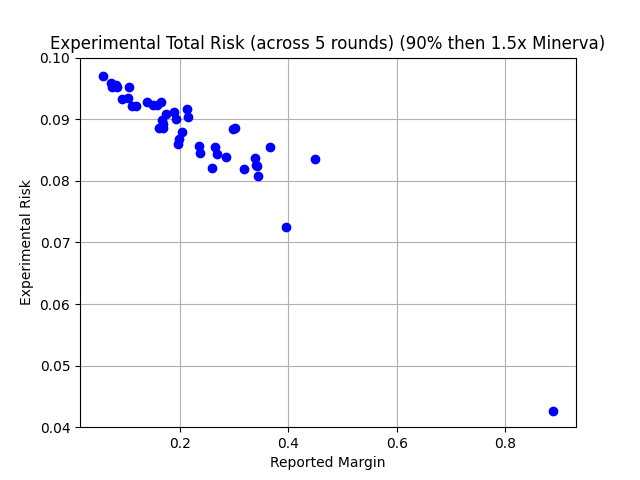
\includegraphics[scale=.7]{minerva_multiround_1p5x_10^6/total_risk.png}




\end{document}

